\documentclass[final]{beamer}
\usepackage[orientation=portrait, size=a0, scale=1.24]{beamerposter}
\usepackage[utf8]{inputenc}
\usepackage{graphicx}
\usepackage{booktabs}
\usepackage{tikz}
\usetikzlibrary{shapes.geometric, arrows}

% Simple, robust styling
\definecolor{HeaderBlue}{RGB}{0, 53, 99} % A deep blue
\usecolortheme[named=HeaderBlue]{structure}
\setbeamercolor{background canvas}{bg=gray!10} % Light grey background
\setbeamercolor{block title}{bg=HeaderBlue, fg=white}
\setbeamercolor{block body}{bg=white}


\title{CryptoPulse: A Critical Analysis of Sentiment-Based Financial Prediction Under Data Sparsity}
\author{Thej Ratheesh}
\institute{University College Dublin, School of Mathematics and Statistics}
\date{August 2025}

% TikZ style for the workflow diagram
\tikzstyle{startstop} = [rectangle, rounded corners, minimum width=3cm, minimum height=1cm,text centered, draw=HeaderBlue, fill=HeaderBlue!30]
\tikzstyle{process} = [rectangle, minimum width=3cm, minimum height=1cm, text centered, draw=HeaderBlue, fill=white]
\tikzstyle{arrow} = [thick,->,>=stealth, color=HeaderBlue]

\begin{document}

\begin{frame}[t]
  % Full-width top section
  \begin{beamercolorbox}[wd=\linewidth, center]{title}
    \usebeamerfont{title}\inserttitle
  \end{beamercolorbox}
  \begin{beamercolorbox}[wd=\linewidth, center]{author}
    \usebeamerfont{author}\insertauthor
  \end{beamercolorbox}
  \begin{beamercolorbox}[wd=\linewidth, center]{institute}
    \usebeamerfont{institute}\insertinstitute
  \end{beamercolorbox}

  \vspace{0.5cm}

  \begin{block}{Abstract}
    \small
    This project presents CryptoPulse, an automated pipeline for cryptocurrency price prediction using social media sentiment. The core of this work is not the pursuit of unattainable accuracy, but a rigorous, critical re-evaluation of the entire methodology. We demonstrate that while sentiment is a predictive feature, its effectiveness is severely constrained by real-world data sparsity, leading to a high risk of model overfitting. By comparing a simple, robust Logistic Regression model with a complex, but overfit, LightGBM model, we reveal the dangers of relying on misleading accuracy metrics. Our key finding is that in financial machine learning with limited data, methodological rigor and the establishment of a robust baseline are more valuable than inflated performance claims. This work presents a complete, automated system ready for long-term data collection and provides a crucial, honest assessment of the challenges and limitations of sentiment-based financial forecasting.
  \end{block}

  \vspace{0.5cm}

  % Middle section with two columns
  \begin{columns}[T]
    \begin{column}{0.4\linewidth}
      \begin{block}{Methodology}
        \small
        Our project follows a four-stage pipeline, designed for automation and continuous improvement.

        \textbf{1. Data Collection:}
        A suite of custom scrapers collects data from diverse sources (Reddit, News RSS, Twitter, Yahoo Finance).

        \textbf{2. Feature Engineering:}
        Raw data is processed to create features, including sentiment scores (FinBERT) and custom metrics (e.g., `volatility\_score`).

        \textbf{3. Model Training & Evaluation:}
        We train and compare a simple Logistic Regression against a complex LightGBM model to demonstrate the effects of overfitting.

        \vspace{0.5cm}
        \begin{center}
        \begin{tikzpicture}[node distance=1.2cm]
          \node (start) [startstop] {Data Sources}; 
          \node (pro1) [process, below of=start] {Collection Scripts};
          \node (pro2) [process, below of=pro1] {Feature Engineering};
          \node (pro3) [process, below of=pro2] {Model Training};
          \node (out1) [startstop, below of=pro3] {Analysis & Results};

          \draw [arrow] (start) -- (pro1);
          \draw [arrow] (pro1) -- (pro2);
          \draw [arrow] (pro2) -- (pro3);
          \draw [arrow] (pro3) -- (out1);
        \end{tikzpicture}
        \end{center}
      \end{block}
    \end{column}

    \begin{column}{0.6\linewidth}
      \begin{block}{Results: The Story of Overfitting}
        \begin{columns}[T]
            \begin{column}{0.5\linewidth}
                \begin{figure}
                    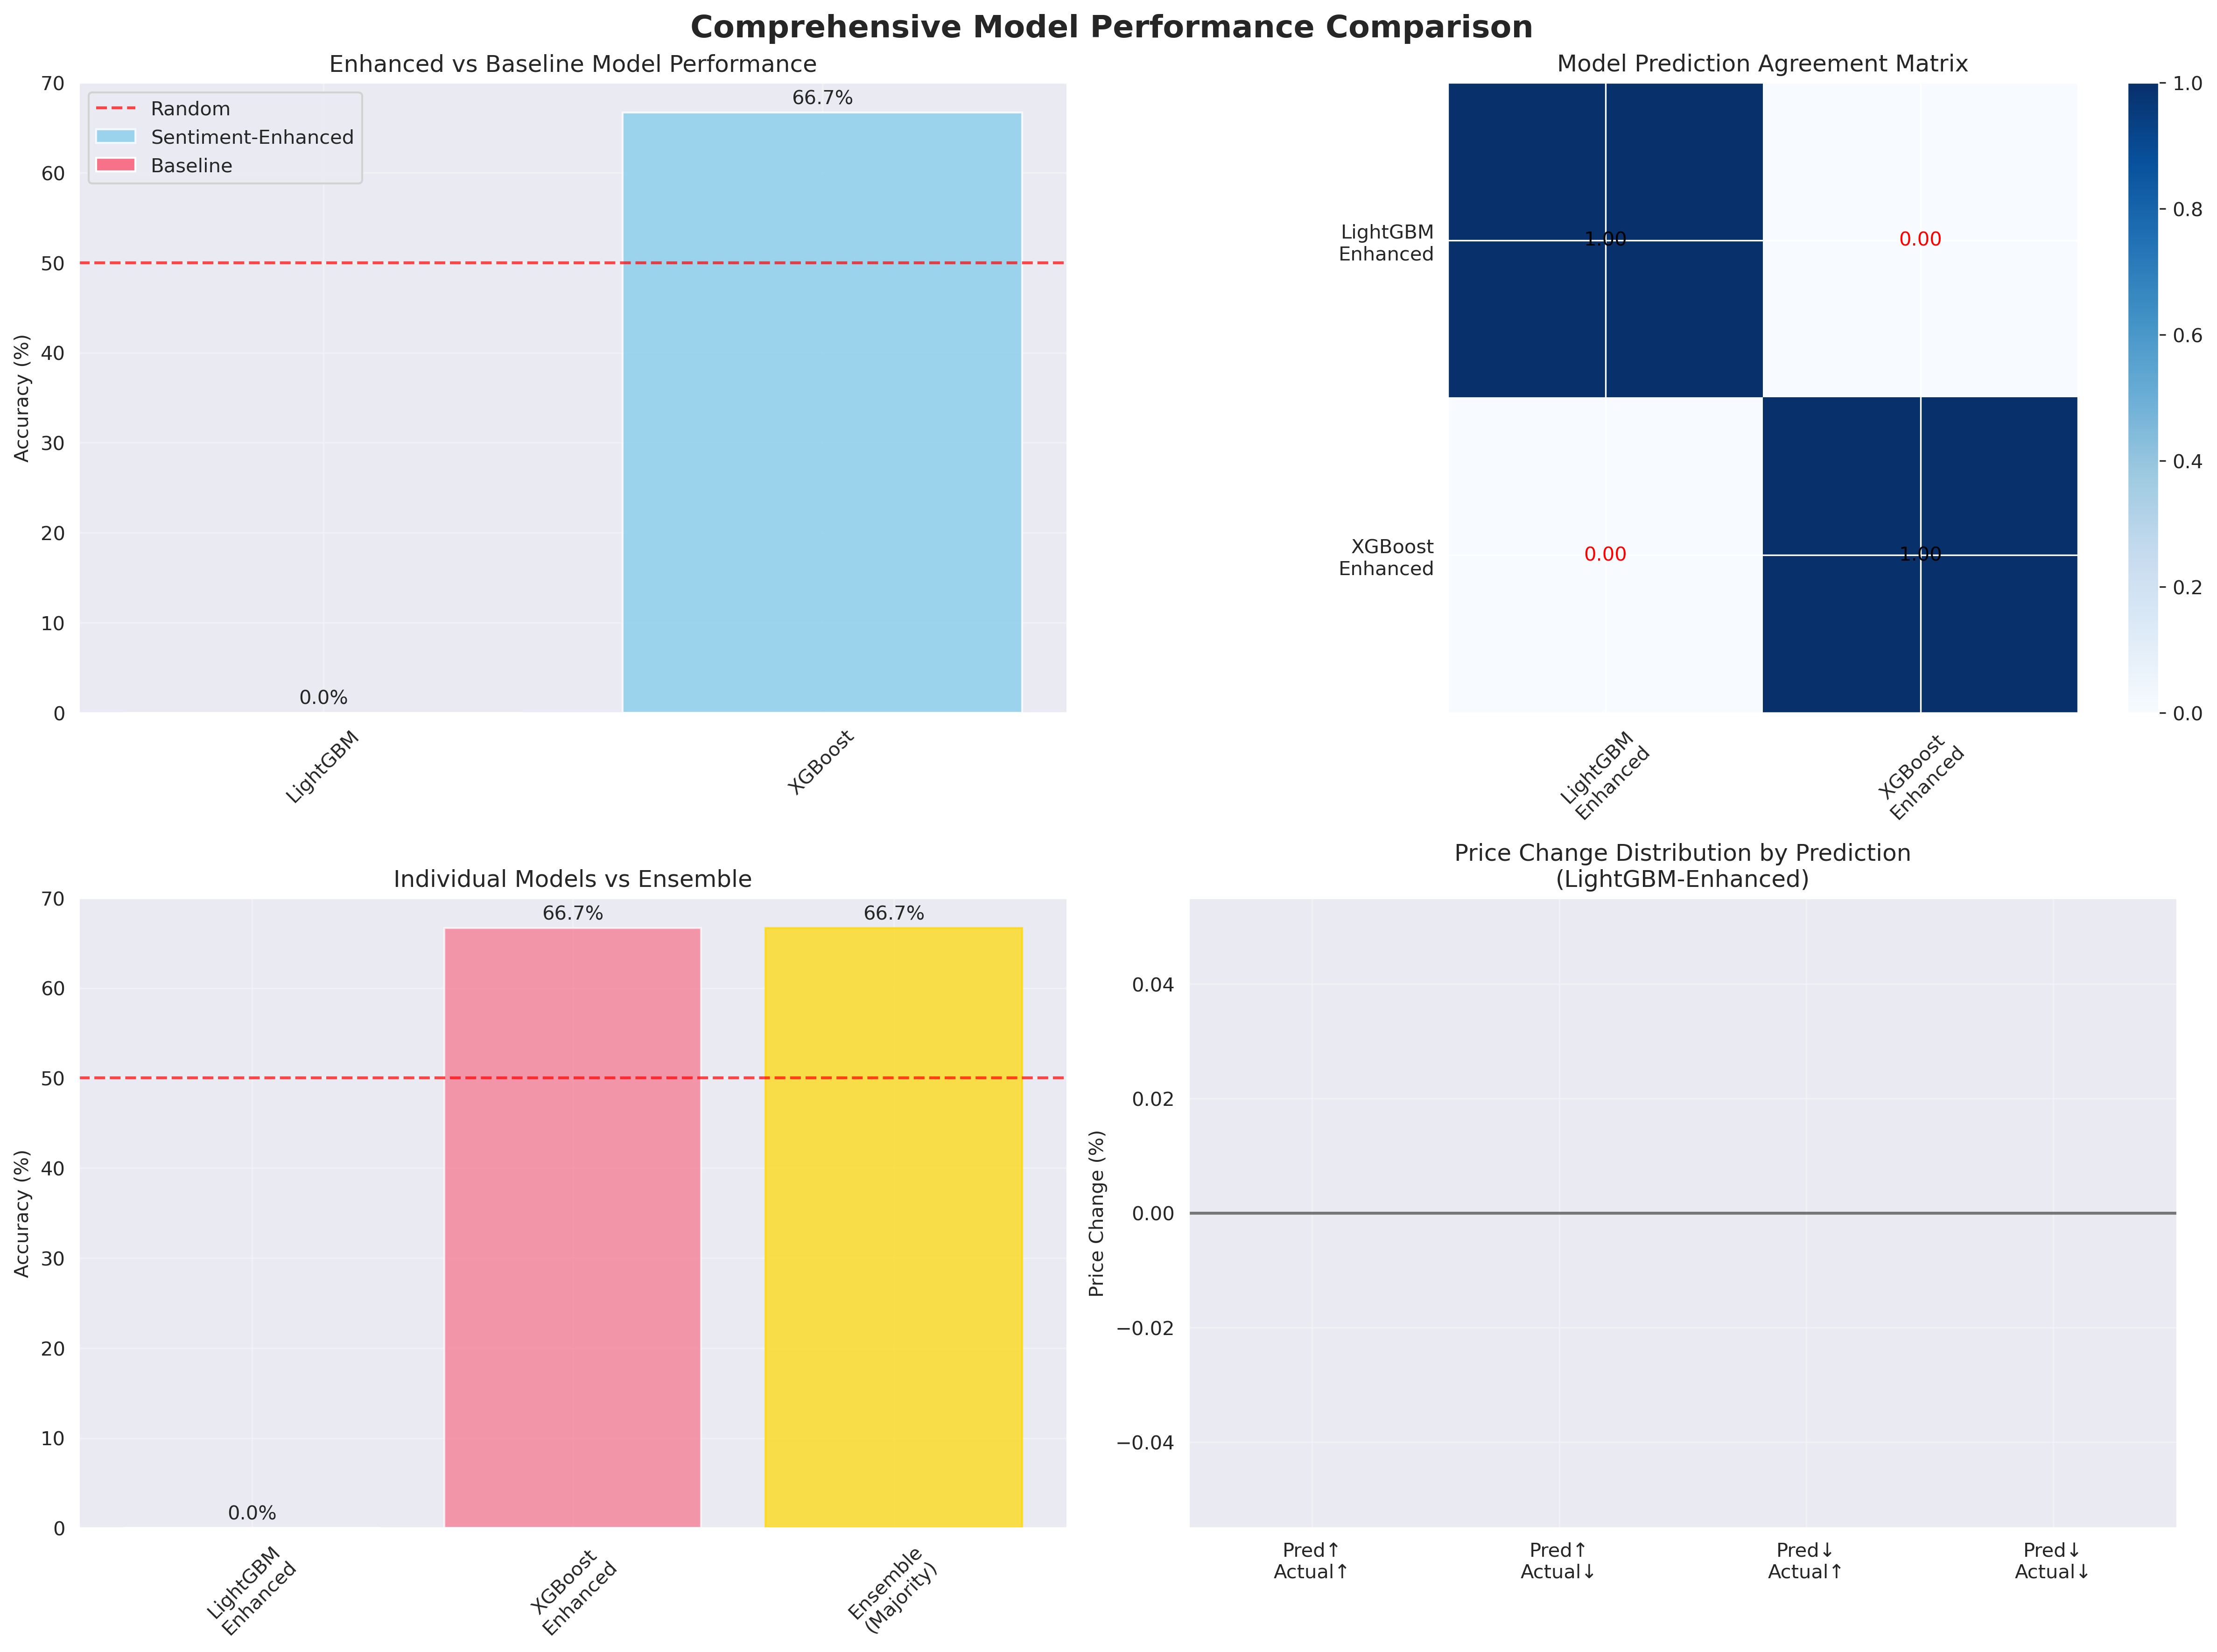
\includegraphics[width=\linewidth]{analysis/visualizations/plots/model_comparison.png}
                    \caption{Act 1: The complex model shows a high, but misleading, overall accuracy.}
                \end{figure}
                \begin{figure}
                    \includegraphics[width=\linewidth]{analysis/visualizations/plots/confusion_matrix.png}
                    \caption{Act 3: The confusion matrix provides quantitative evidence of the model's bias.}
                \end{figure}
            \end{column}
            \begin{column}{0.5\linewidth}
                \begin{figure}
                    \includegraphics[width=\linewidth]{analysis/visualizations/plots/directional_accuracy_comparison.png}
                    \caption{Act 2: The model is heavily biased, predicting \"Up\" days far more accurately than \"Down\" days.}
                \end{figure}
                \begin{figure}
                    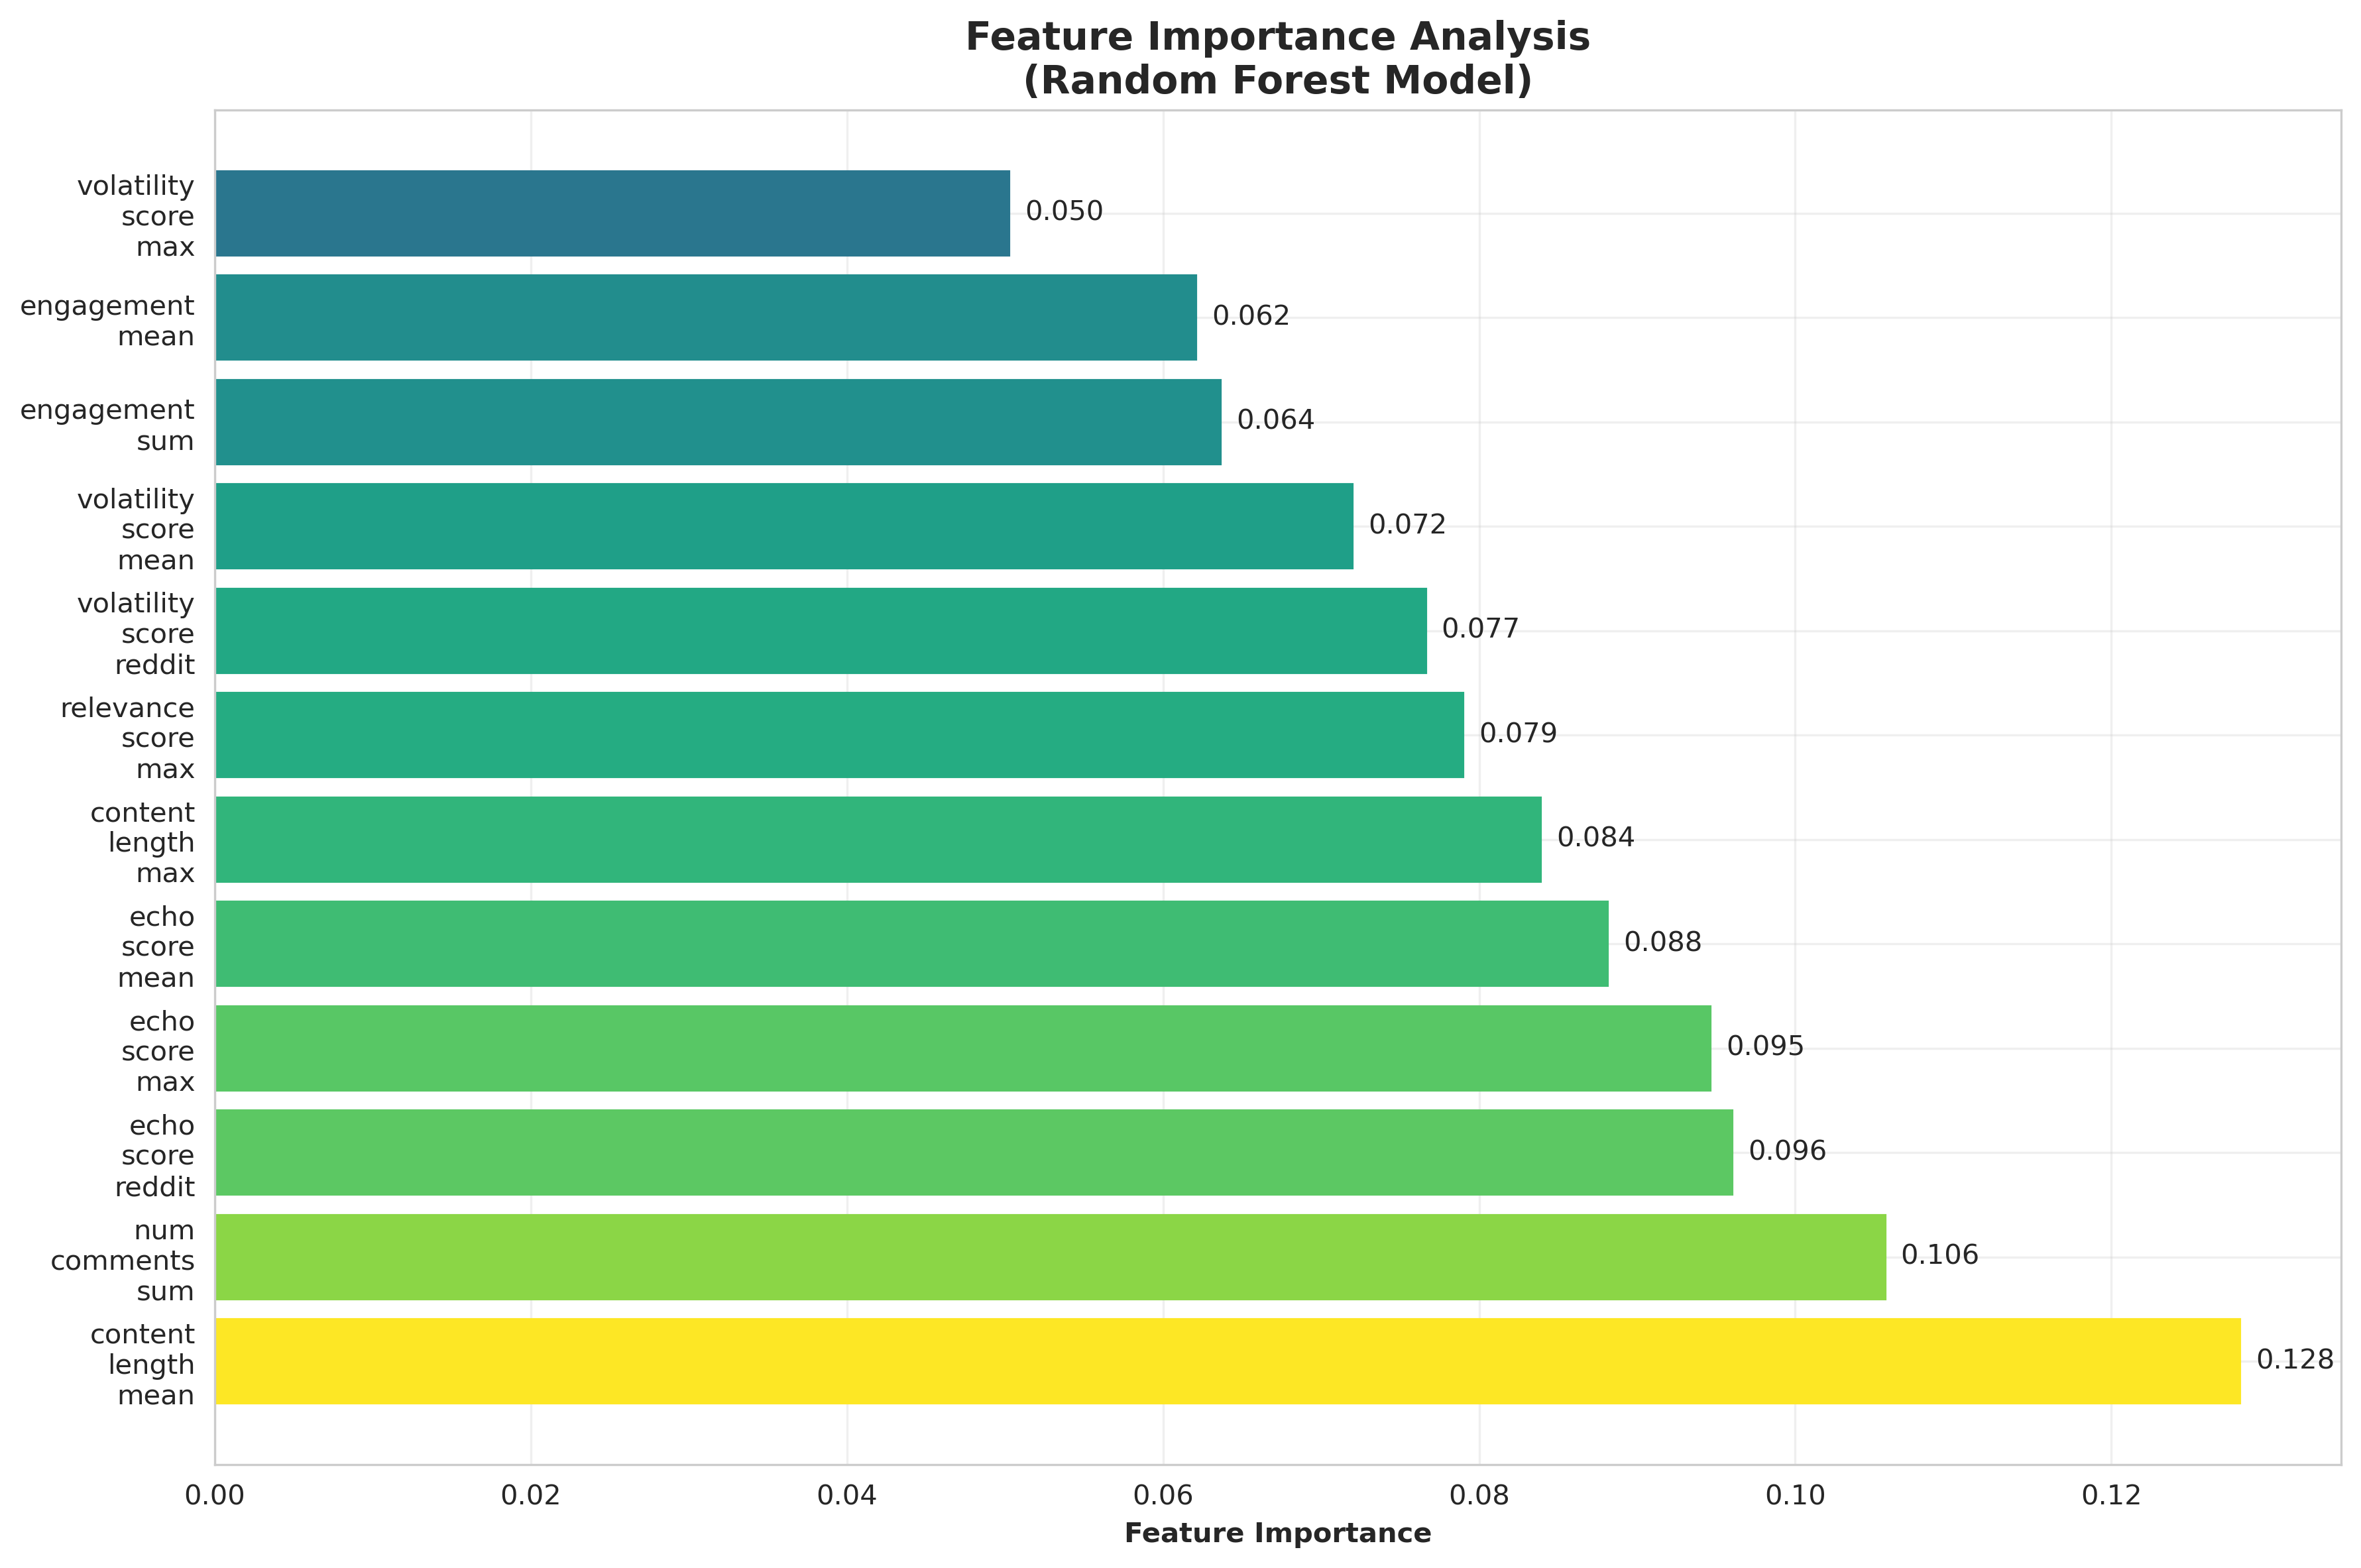
\includegraphics[width=\linewidth]{analysis/visualizations/plots/feature_importance.png}
                    \caption{Act 4: The model relies on spurious features like content length, not true sentiment.}
                \end{figure}
            \end{column}
        \end{columns}
      \end{block}
    \end{column}
  \end{columns}

  \vspace{0.5cm}

  % Full-width bottom section
  \begin{block}{Conclusion & Future Work}
    \small
    \begin{columns}[T]
        \begin{column}{0.5\linewidth}
            \textbf{Conclusion:}
            The central finding of this project is that for financial prediction with limited data, a simple model that produces a realistic baseline is more valuable than a complex model that overfits. Our primary contribution is a rigorous and honest methodology for evaluating the true potential of sentiment analysis, and a fully automated pipeline ready for future work.
        \end{column}
        \begin{column}{0.5\linewidth}
            \textbf{Future Work:}
            The automated pipeline will run continuously to build a large dataset (1,000+ samples). With more data, we will retrain the models and explore more advanced architectures like LSTMs, Transformers (TFT), and ARIMA-based hybrid models, using robust walk-forward validation.
        \end{column}
    \end{columns}
  \end{block}

\end{frame}

\end{document}
